\documentclass[11pt,a4paper]{article}

\usepackage[a4paper,margin=2.2cm]{geometry}
\usepackage[T1]{fontenc}
\usepackage{lmodern}
\usepackage[utf8]{inputenc}
\usepackage{microtype}
\usepackage{amsmath}
\usepackage{graphicx}
\usepackage{booktabs}
\usepackage{xcolor}
\usepackage{listings}
\usepackage{enumitem}
\usepackage{caption}
\usepackage{float}
\usepackage{parskip}
\usepackage[colorlinks=true,linkcolor=accent,urlcolor=accent]{hyperref}

\definecolor{accent}{RGB}{31,78,121}
\definecolor{codebg}{RGB}{246,247,249}
\definecolor{codeframe}{RGB}{215,218,224}
\definecolor{kw}{RGB}{0,92,170}
\definecolor{cm}{RGB}{110,120,130}
\definecolor{st}{RGB}{163,21,21}
\definecolor{bad}{RGB}{190,40,40}
\definecolor{good}{RGB}{30,130,60}
\definecolor{boxbg}{RGB}{236,242,249}

\lstset{
  language=Python,
  basicstyle=\ttfamily\small,
  keywordstyle=\color{kw}\bfseries,
  commentstyle=\color{cm}\itshape,
  stringstyle=\color{st},
  backgroundcolor=\color{codebg},
  frame=single, rulecolor=\color{codeframe},
  framesep=4pt, xleftmargin=6pt, xrightmargin=6pt,
  breaklines=true, showstringspaces=false,
  columns=fullflexible, keepspaces=true,
  numbers=none, aboveskip=8pt, belowskip=8pt,
  literate={×}{{$\times$}}1 {→}{{$\rightarrow$}}1 {σ}{{$\sigma$}}1 {~}{{$\sim$}}1,
}

\newcommand{\keybox}[1]{%
  \par\noindent\colorbox{boxbg}{\parbox{\dimexpr\linewidth-2\fboxsep}{\vspace{4pt}#1\vspace{4pt}}}\par}

\captionsetup{font=small,labelfont=bf}

\title{\color{accent}\textbf{Data leakage in the CNN denoising project}\\[4pt]
\large What went wrong in v1, how to prove it, and how v2 fixes it}
\author{}
\date{November 2026}

\begin{document}
\maketitle
\vspace{-1em}

\keybox{\textbf{Summary.}
The 1000 ``different'' MRI images in v1 are really \textbf{10 distinct slices, each copied 100 times}, because the
phantom does not change over time. The random 80/20 split therefore put about 80 near-identical copies of
every validation image into the training set. The validation score measured how well the network
\emph{remembers} slices it has already seen, not how well it denoises new ones.

An experiment with fresh noise shows the effect directly. Both the v1 and the v2 model beat a Gaussian filter by
about \textbf{5 dB on slices they trained on, but only about 3 dB on slices they never saw}. v2 fixes the leak by
splitting on slice position, adding buffer slices, normalising using training data only, and keeping a
separate test set.}

\section{What data leakage is}

A model is supposed to be judged on data it has never seen, because that is the situation it will face in practice.
\textbf{Leakage} is when information about the evaluation data gets into training anyway. The evaluation then
measures something easier than the real task, and the number looks better than it really is.

An exam analogy: if the exam questions are the homework questions with the numbers slightly changed, a high score
shows that the student remembers the homework, not that they understand the subject.

The key question to ask in any project is:
\begin{quote}
\emph{What is the real unit of independence in my data?}
\end{quote}
In medical imaging it is almost never the individual image. It is usually the patient, the scan, or (here) the
anatomical position. Two images from the same unit are not independent, and they must stay on the same
side of the split.

\section{How v1 built the dataset}

\texttt{make\_dataset.py} in v1 takes a 4D EPI volume (64\,$\times$\,64 pixels, 30 slices, 300 timepoints),
keeps the first 100 timepoints, and takes the 10 central slices from each:

\begin{lstlisting}
V = V[..., :100]                         # (64, 64, 30, 100)

slices = []
for t in range(V.shape[3]):              # 100 timepoints
    for z in range(10, V.shape[2]-10):   # z = 10..19  (10 slice positions)
        slices.append(V[:, :, z, t])

X_clean = np.stack(slices, axis=0)       # (1000, 64, 64)
\end{lstlisting}

So far this looks like 1000 images. The catch is in what a ``timepoint'' means for this data.

\section{The catch: the phantom does not change over time}

The data is a BOLD fMRI time series of a \emph{phantom}, a static plastic object, not a living brain. Nothing
changes from one timepoint to the next until the robot moves it at around timepoint 146. Figure~\ref{fig:time}
shows the same slice at the first and last timepoint used:

\begin{figure}[H]
  \centering
  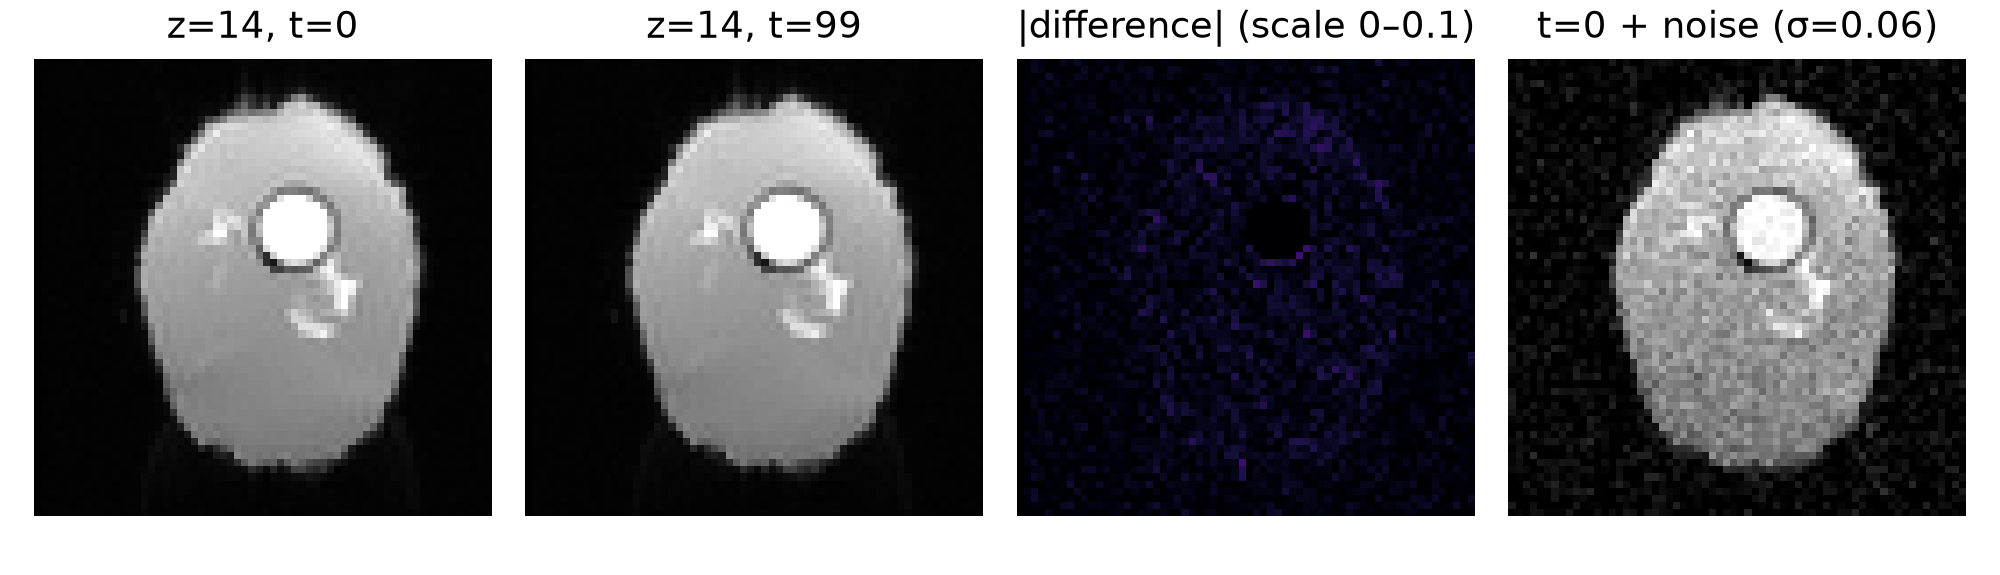
\includegraphics[width=\linewidth]{figs/fig_time.png}
  \caption{Slice $z=14$ at $t=0$ and $t=99$. The difference map (third panel) is almost black: the mean absolute
  difference is $0.0036$, about $17\times$ smaller than the synthetic noise ($\sigma=0.06$, fourth panel).
  The pixel-wise correlation between the two images is $0.99993$.}
  \label{fig:time}
\end{figure}

\keybox{So the dataset is not 1000 different images. It is \textbf{10 different images} (one per slice position
$z=10\ldots19$), each repeated 100 times with tiny differences, and each repeat given its own random noise.}

\section{How v1 split the data, and why that leaks}

\texttt{train\_autoencoder.py} in v1 splits by shuffling \emph{image indices}:

\begin{lstlisting}
idx = torch.randperm(len(X_clean))        # shuffle all 1000 images
split = int(0.8 * len(idx))
train_idx, val_idx = idx[:split], idx[split:]
\end{lstlisting}

Take any validation image, say slice $z=14$ at $t=37$. There are 99 other images of slice 14, and about 80\%
of them (\textbf{$\sim$79 images}) are in the training set. The training targets for those images are clean
versions of slice 14 that are 99.99\% identical to the validation target.

Over hundreds of epochs the network sees the clean slice 14 roughly 80 times per epoch. A network trained like
this can learn a shortcut: \emph{``this noisy image looks like slice 14, so output the slice 14 I remember''}.
That shortcut gives excellent validation scores and fails on any slice it has not seen.

\paragraph{``But the noise is different in every image, so isn't that fine?''}
Partly. The noise realisations are different, so the network cannot simply memorise noisy--clean pairs.
However, the \emph{clean target} is what the network has to produce, and that is the part it has seen
many times. Denoising is hard because the network must guess what the clean image underneath looks like.
Leakage gives it the answer to that guess.

\paragraph{A second, smaller leak in v1.}
\texttt{use\_trained\_autencoder.py} calls \texttt{torch.randperm} again with no fixed seed, so its
``validation'' images are a \emph{new} random 20\%, most of which were in the training set of the loaded model.
The example figures it produces are mostly images the model was trained on.

\section{Proving it: seen versus unseen slices}

Claiming leakage is easy, so it is worth measuring. v1 trained on $z=10\ldots19$ but the volume has phantom
content on $z=3\ldots24$, so there are 12 slice positions the v1 model has never seen. The test is to give
every slice \textbf{fresh} noise (a new random seed, so no image is reused) and measure PSNR.

There is one complication: some slices are naturally easier to denoise than others (for example, smaller
cross-sections with more empty background). To remove that effect, each slice is also denoised with a
Gaussian filter, and we look at the \textbf{CNN's gain over the Gaussian filter} on that same slice. A
Gaussian filter has no training, so it measures how hard the slice is without any memorisation.

\begin{lstlisting}
for z in range(3, 25):
    clean = np.stack([V[:, :, z, t] for t in range(0, 100, 5)])      # 20 timepoints
    noise = 0.06 * rng.standard_normal(clean.shape)                 # FRESH noise
    noisy = np.clip(clean + noise, 0, 1)
    gauss = np.stack([gaussian_filter(x, 0.6) for x in noisy])
    cnn   = model(torch.from_numpy(noisy[:, None]).float()).numpy()[:, 0]
    gain[z] = psnr(cnn, clean) - psnr(gauss, clean)                  # in dB
\end{lstlisting}

The same experiment was run on the v2 model, which trained on a \emph{different} set of slices.

\begin{figure}[H]
  \centering
  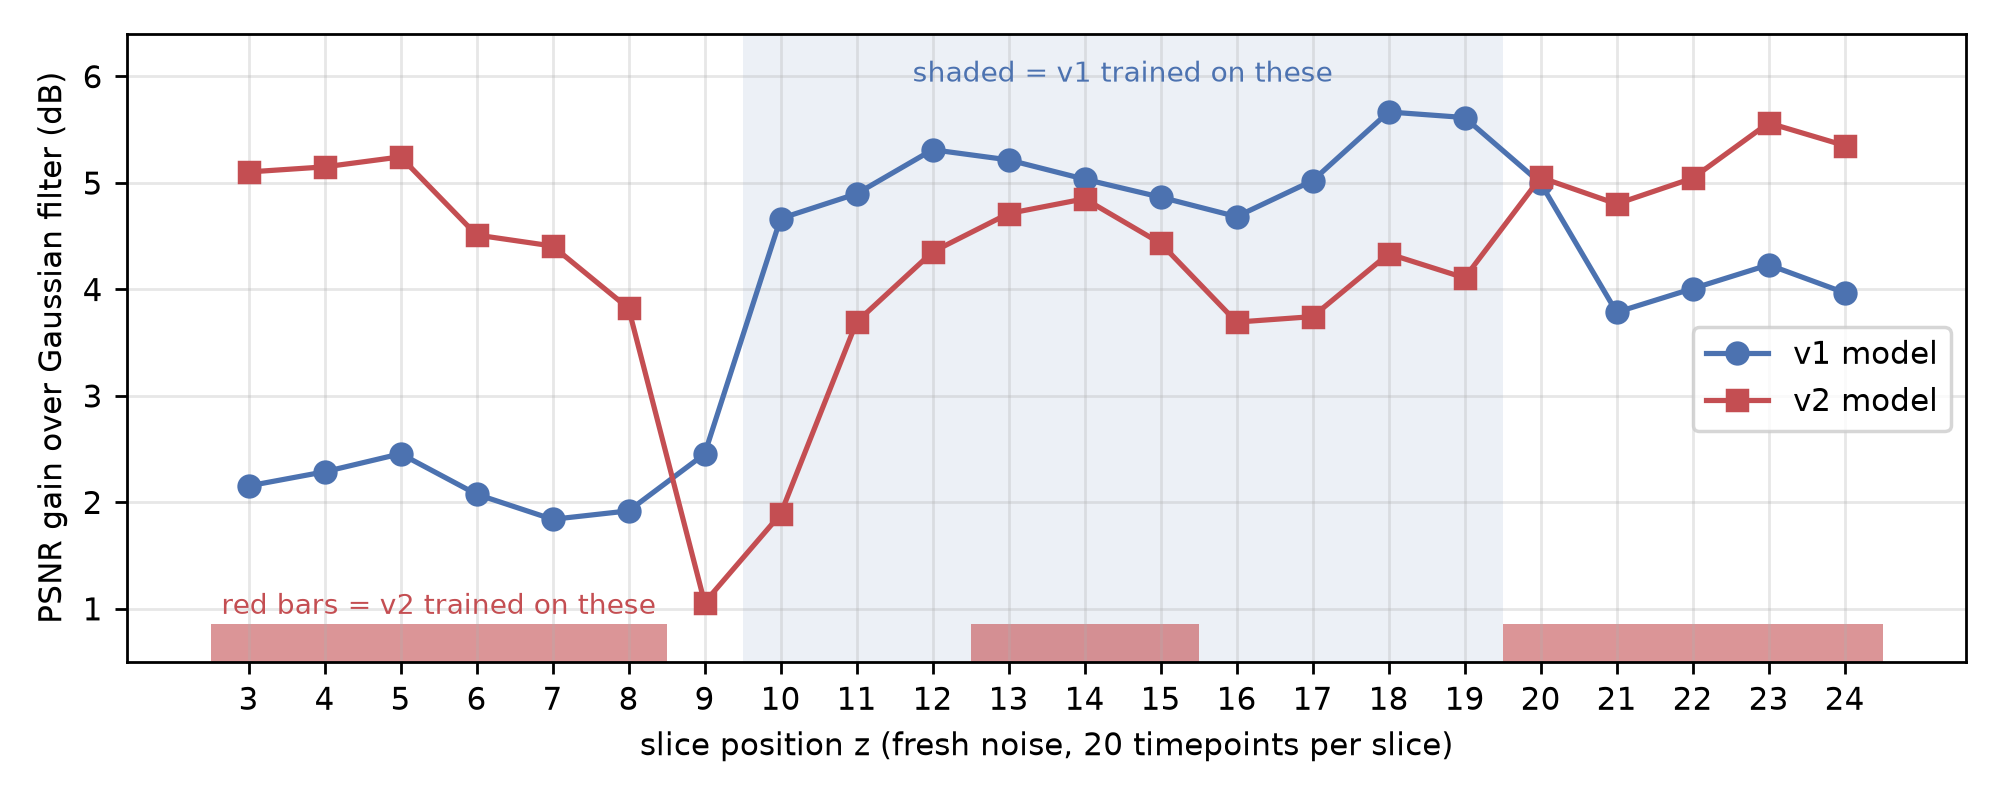
\includegraphics[width=\linewidth]{figs/fig_crossover.png}
  \caption{CNN gain over a Gaussian filter, per slice, with fresh noise. Blue (v1) is high inside the shaded
  region it trained on and drops outside it. Red (v2) is high on its own training slices (red bars) and lower
  in between. Each model is best on whatever slices it was trained on.}
  \label{fig:cross}
\end{figure}

\begin{table}[H]
  \centering
  \begin{tabular}{lcc}
    \toprule
    & \multicolumn{2}{c}{mean gain over Gaussian filter (dB)} \\
    \cmidrule(lr){2-3}
    model & slices it trained on & slices it never saw \\
    \midrule
    v1 (1000 epochs, $z=10\ldots19$) & \textbf{5.10} & 3.01 \\
    v2 (300 epochs, see Section~\ref{sec:fix}) & \textbf{4.86} & 3.36 \\
    \bottomrule
  \end{tabular}
  \caption{Both models are about 2 dB better on slices they have seen, even though the noise is new.}
  \label{tab:gap}
\end{table}

The clearest evidence is the \textbf{crossover}. At $z=5$ the v2 model (which trained there) is 5.2 dB ahead
of the filter and v1 only 2.5 dB. At $z=10$ it is reversed: v1 is 4.7 dB ahead and v2 only 1.9 dB. Nothing about
the slice changed, only which model had seen it.

\keybox{\textbf{What this means for v1's reported number.}
v1's final validation MSE was about $4.5\times10^{-4}$, which is
$10\log_{10}(1/4.5\times10^{-4}) \approx 33.5$ dB. That matches its PSNR on \emph{seen} slices ($\approx 33.7$ dB),
not on unseen ones. The validation score was really a score on the training data.}

Note that v2 also does better on its own training slices; every model does. That is normal and is called the
\emph{generalisation gap}. Leakage is not that the gap exists, but that v1's evaluation was on the wrong side of it,
so the gap was invisible.

\section{The fix in v2}
\label{sec:fix}

\subsection{Split by slice position, not by image}

Each slice position $z$ is assigned to exactly one of train, validation or test. All 100 timepoints of a slice
go to the same split, so copies of one image can never be on both sides.

\begin{lstlisting}
VAL_Z    = [10, 11]
TEST_Z   = [17, 18]
BUFFER_Z = [9, 12, 16, 19]            # unused: separate val/test from train
TRAIN_Z  = [z for z in range(3, 25) if z not in VAL_Z + TEST_Z + BUFFER_Z]

for name, zlist in (("train", TRAIN_Z), ("val", VAL_Z), ("test", TEST_Z)):
    for z in zlist:
        for t in range(N_TIME):
            clean.append(V[:, :, z, t])
            split.append(name)        # the split label is stored with every image
\end{lstlisting}

\begin{figure}[H]
  \centering
  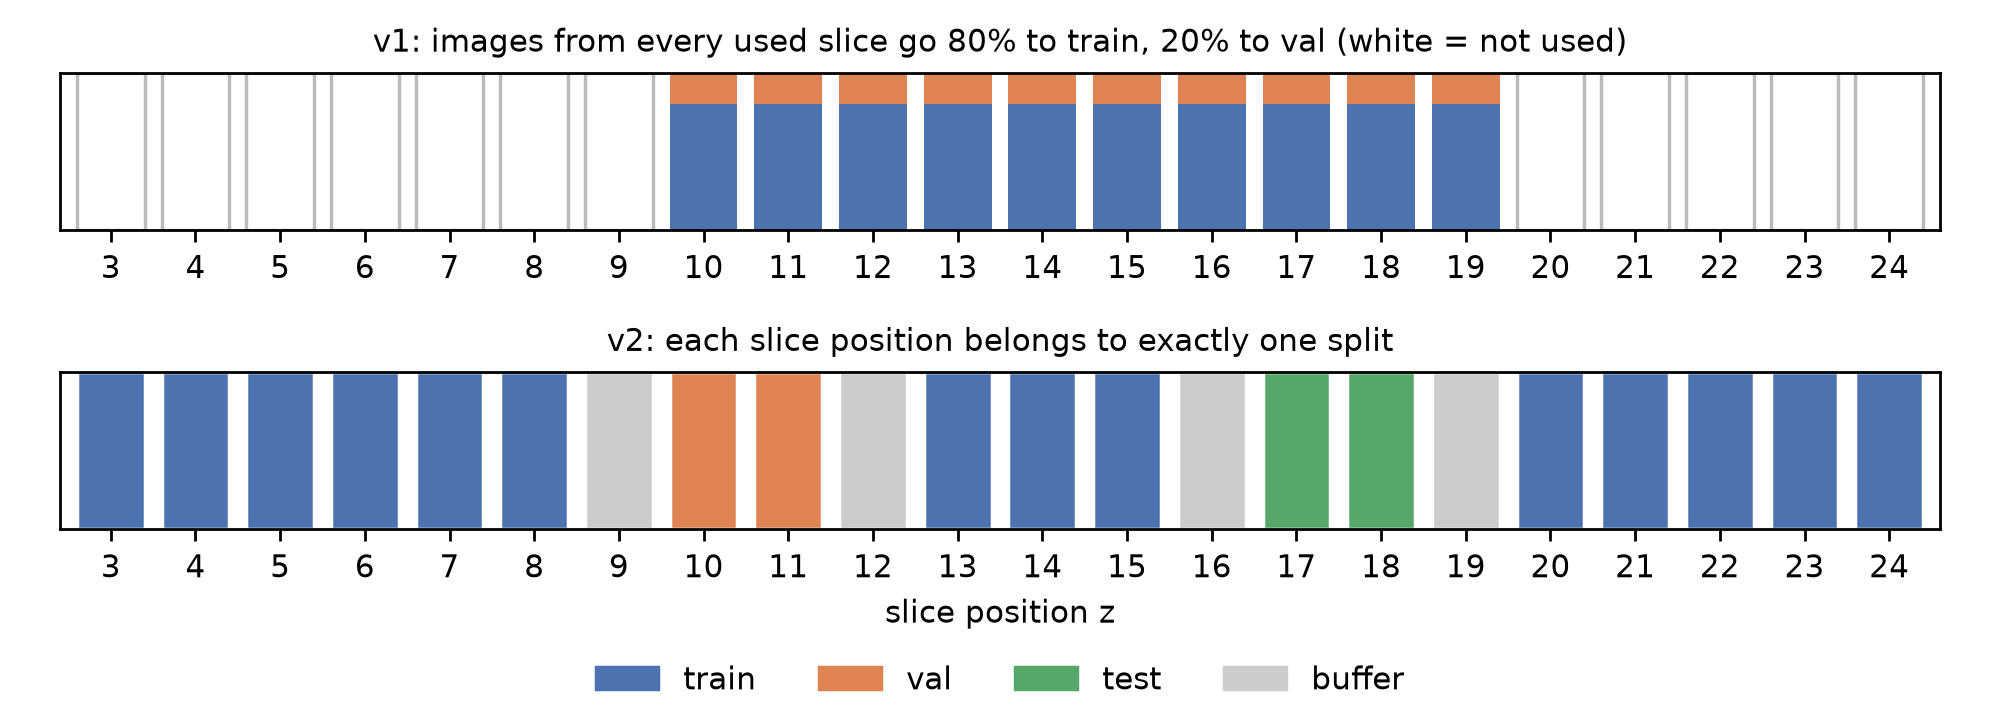
\includegraphics[width=\linewidth]{figs/fig_split.png}
  \caption{v1 versus v2 split. In v1 every slice appears in both train and validation. In v2 each slice belongs to
  one split, and grey buffer slices are left out completely.}
\end{figure}

\subsection{Why the buffer slices}

Neighbouring slices are not independent either. Slices are 4.2 mm apart, so anatomy changes
gradually. The average correlation between slices $d$ positions apart is:

\begin{center}
\begin{tabular}{lcccc}
  \toprule
  distance $d$ & 1 & 2 & 3 & 5 \\
  \midrule
  correlation & 0.961 & 0.909 & 0.868 & 0.802 \\
  \bottomrule
\end{tabular}
\end{center}

Without buffers, validation slice 10 would sit right next to training slice 9 and be 96\% similar to it.
The buffers make the closest training slice two positions away. This is a compromise: more buffer means less
leakage but less training data, and with only 22 usable slices that trade-off is tight.

\subsection{Normalise using training data only}

v1 computed the intensity-scaling percentiles over the whole volume, including the evaluation slices:

\begin{lstlisting}
vmin, vmax = np.percentile(V, (1, 99))                       # v1: all slices
vmin, vmax = np.percentile(V[:, :, TRAIN_Z, :], (1, 99))     # v2: training slices only
\end{lstlisting}

Here the effect is tiny, but the rule matters: \textbf{any value estimated from data (scaling, means, PCA,
feature selection, thresholds) must be estimated from the training set only}, then applied unchanged to
validation and test. Otherwise the evaluation data has influenced the model.

\subsection{Separate validation and test}

Every decision made by looking at a dataset leaks a little information from it. In v2, validation is used to
\begin{itemize}[nosep]
  \item pick the best checkpoint (the epoch with the lowest validation MSE), and
  \item tune the Gaussian filter's $\sigma$ (so the baseline is fair),
\end{itemize}
which makes the validation score slightly optimistic. The \textbf{test} slices are used once, at the end,
for the reported numbers.

\subsection{One split, stored with the data}

The split label is saved inside the \texttt{.npz} file, and every script loads it through one function, so
training and evaluation always agree on which images are which:

\begin{lstlisting}
def load_split(name):                      # 'train', 'val' or 'test'
    D = np.load(DATA_NPZ)
    m = D["split"] == name
    noisy = torch.from_numpy(D["noisy"][m][:, None])
    clean = torch.from_numpy(D["clean"][m][:, None])
    return noisy, clean
\end{lstlisting}

\section{Honest results}

On the held-out test slices ($z=17,18$; 200 images):

\begin{center}
\begin{tabular}{lccc}
  \toprule
  method & MSE & PSNR (dB) & SSIM \\
  \midrule
  noisy input            & 0.00249 & 26.04 & 0.622 \\
  Gaussian filter ($\sigma=0.6$) & 0.00149 & 28.28 & 0.756 \\
  CNN, skip connection (300 ep.) & \textbf{0.00061} & \textbf{32.14} & \textbf{0.935} \\
  CNN, no skip (300 ep.) & 0.00071 & 31.49 & 0.932 \\
  \bottomrule
\end{tabular}
\end{center}

The CNN still clearly works: it gains about 6 dB over the noisy input and 4 dB over a tuned Gaussian filter on
anatomy it has never seen. The result is a little lower than v1's number, but it can be trusted.

\paragraph{What the fix does not solve.}
All splits still come from \emph{one phantom in one scan}. The test measures generalisation to unseen
cross-sections of the same object, not to new subjects, scanners or noise levels. That would need more scans,
and with more scans the split should be \emph{by scan} (or by subject).

\section{Checklist for future projects}

\begin{enumerate}[leftmargin=*]
  \item \textbf{Find the unit of independence} (patient, scan, slice position, time window) and split on it.
        In scikit-learn this is \texttt{GroupShuffleSplit} or \texttt{GroupKFold}, where the group is that unit.
  \item \textbf{Look for near-duplicates.} Before trusting ``N images'', check how many are actually different,
        for example by computing correlations between images.
  \item \textbf{Leave a gap} around the evaluation data when neighbouring samples are correlated (adjacent
        slices, neighbouring time windows in a time series).
  \item \textbf{Split before preprocessing}, and fit every normalisation or transform on training data only.
  \item \textbf{Keep a test set you touch once.} Use validation for decisions and test for the final number.
  \item \textbf{Save the split} with the data (or fix the random seed), so every script uses the same one.
  \item \textbf{Be suspicious of results that look too good}, and test the suspicion directly with an experiment
        like the seen/unseen comparison in Section 5.
\end{enumerate}

\end{document}
